\documentclass{ximera}

%\usepackage{todonotes}
%\usepackage{mathtools} %% Required for wide table Curl and Greens
%\usepackage{cuted} %% Required for wide table Curl and Greens
\newcommand{\todo}{}

\usepackage{esint} % for \oiint
\ifxake%%https://math.meta.stackexchange.com/questions/9973/how-do-you-render-a-closed-surface-double-integral
\renewcommand{\oiint}{{\large\bigcirc}\kern-1.56em\iint}
\fi


\graphicspath{
  {./}
  {ximeraTutorial/}
  {basicPhilosophy/}
  {functionsOfSeveralVariables/}
  {normalVectors/}
  {lagrangeMultipliers/}
  {vectorFields/}
  {greensTheorem/}
  {shapeOfThingsToCome/}
  {dotProducts/}
  {partialDerivativesAndTheGradientVector/}
  {../productAndQuotientRules/exercises/}
  {../normalVectors/exercisesParametricPlots/}
  {../continuityOfFunctionsOfSeveralVariables/exercises/}
  {../partialDerivativesAndTheGradientVector/exercises/}
  {../directionalDerivativeAndChainRule/exercises/}
  {../commonCoordinates/exercisesCylindricalCoordinates/}
  {../commonCoordinates/exercisesSphericalCoordinates/}
  {../greensTheorem/exercisesCurlAndLineIntegrals/}
  {../greensTheorem/exercisesDivergenceAndLineIntegrals/}
  {../shapeOfThingsToCome/exercisesDivergenceTheorem/}
  {../greensTheorem/}
  {../shapeOfThingsToCome/}
  {../separableDifferentialEquations/exercises/}
  {vectorFields/}
}

\newcommand{\mooculus}{\textsf{\textbf{MOOC}\textnormal{\textsf{ULUS}}}}

\usepackage{tkz-euclide}\usepackage{tikz}
\usepackage{tikz-cd}
\usetikzlibrary{arrows}
\tikzset{>=stealth,commutative diagrams/.cd,
  arrow style=tikz,diagrams={>=stealth}} %% cool arrow head
\tikzset{shorten <>/.style={ shorten >=#1, shorten <=#1 } } %% allows shorter vectors

\usetikzlibrary{backgrounds} %% for boxes around graphs
\usetikzlibrary{shapes,positioning}  %% Clouds and stars
\usetikzlibrary{matrix} %% for matrix
\usepgfplotslibrary{polar} %% for polar plots
\usepgfplotslibrary{fillbetween} %% to shade area between curves in TikZ
\usetkzobj{all}
\usepackage[makeroom]{cancel} %% for strike outs
%\usepackage{mathtools} %% for pretty underbrace % Breaks Ximera
%\usepackage{multicol}
\usepackage{pgffor} %% required for integral for loops



%% http://tex.stackexchange.com/questions/66490/drawing-a-tikz-arc-specifying-the-center
%% Draws beach ball
\tikzset{pics/carc/.style args={#1:#2:#3}{code={\draw[pic actions] (#1:#3) arc(#1:#2:#3);}}}



\usepackage{array}
\setlength{\extrarowheight}{+.1cm}
\newdimen\digitwidth
\settowidth\digitwidth{9}
\def\divrule#1#2{
\noalign{\moveright#1\digitwidth
\vbox{\hrule width#2\digitwidth}}}





\newcommand{\RR}{\mathbb R}
\newcommand{\R}{\mathbb R}
\newcommand{\N}{\mathbb N}
\newcommand{\Z}{\mathbb Z}

\newcommand{\sagemath}{\textsf{SageMath}}


%\renewcommand{\d}{\,d\!}
\renewcommand{\d}{\mathop{}\!d}
\newcommand{\dd}[2][]{\frac{\d #1}{\d #2}}
\newcommand{\pp}[2][]{\frac{\partial #1}{\partial #2}}
\renewcommand{\l}{\ell}
\newcommand{\ddx}{\frac{d}{\d x}}

\newcommand{\zeroOverZero}{\ensuremath{\boldsymbol{\tfrac{0}{0}}}}
\newcommand{\inftyOverInfty}{\ensuremath{\boldsymbol{\tfrac{\infty}{\infty}}}}
\newcommand{\zeroOverInfty}{\ensuremath{\boldsymbol{\tfrac{0}{\infty}}}}
\newcommand{\zeroTimesInfty}{\ensuremath{\small\boldsymbol{0\cdot \infty}}}
\newcommand{\inftyMinusInfty}{\ensuremath{\small\boldsymbol{\infty - \infty}}}
\newcommand{\oneToInfty}{\ensuremath{\boldsymbol{1^\infty}}}
\newcommand{\zeroToZero}{\ensuremath{\boldsymbol{0^0}}}
\newcommand{\inftyToZero}{\ensuremath{\boldsymbol{\infty^0}}}



\newcommand{\numOverZero}{\ensuremath{\boldsymbol{\tfrac{\#}{0}}}}
\newcommand{\dfn}{\textbf}
%\newcommand{\unit}{\,\mathrm}
\newcommand{\unit}{\mathop{}\!\mathrm}
\newcommand{\eval}[1]{\bigg[ #1 \bigg]}
\newcommand{\seq}[1]{\left( #1 \right)}
\renewcommand{\epsilon}{\varepsilon}
\renewcommand{\phi}{\varphi}


\renewcommand{\iff}{\Leftrightarrow}

\DeclareMathOperator{\arccot}{arccot}
\DeclareMathOperator{\arcsec}{arcsec}
\DeclareMathOperator{\arccsc}{arccsc}
\DeclareMathOperator{\si}{Si}
\DeclareMathOperator{\scal}{scal}
\DeclareMathOperator{\sign}{sign}


%% \newcommand{\tightoverset}[2]{% for arrow vec
%%   \mathop{#2}\limits^{\vbox to -.5ex{\kern-0.75ex\hbox{$#1$}\vss}}}
\newcommand{\arrowvec}[1]{{\overset{\rightharpoonup}{#1}}}
%\renewcommand{\vec}[1]{\arrowvec{\mathbf{#1}}}
\renewcommand{\vec}[1]{{\overset{\boldsymbol{\rightharpoonup}}{\mathbf{#1}}}\hspace{0in}}

\newcommand{\point}[1]{\left(#1\right)} %this allows \vector{ to be changed to \vector{ with a quick find and replace
\newcommand{\pt}[1]{\mathbf{#1}} %this allows \vec{ to be changed to \vec{ with a quick find and replace
\newcommand{\Lim}[2]{\lim_{\point{#1} \to \point{#2}}} %Bart, I changed this to point since I want to use it.  It runs through both of the exercise and exerciseE files in limits section, which is why it was in each document to start with.

\DeclareMathOperator{\proj}{\mathbf{proj}}
\newcommand{\veci}{{\boldsymbol{\hat{\imath}}}}
\newcommand{\vecj}{{\boldsymbol{\hat{\jmath}}}}
\newcommand{\veck}{{\boldsymbol{\hat{k}}}}
\newcommand{\vecl}{\vec{\boldsymbol{\l}}}
\newcommand{\uvec}[1]{\mathbf{\hat{#1}}}
\newcommand{\utan}{\mathbf{\hat{t}}}
\newcommand{\unormal}{\mathbf{\hat{n}}}
\newcommand{\ubinormal}{\mathbf{\hat{b}}}

\newcommand{\dotp}{\bullet}
\newcommand{\cross}{\boldsymbol\times}
\newcommand{\grad}{\boldsymbol\nabla}
\newcommand{\divergence}{\grad\dotp}
\newcommand{\curl}{\grad\cross}
%\DeclareMathOperator{\divergence}{divergence}
%\DeclareMathOperator{\curl}[1]{\grad\cross #1}
\newcommand{\lto}{\mathop{\longrightarrow\,}\limits}

\renewcommand{\bar}{\overline}

\colorlet{textColor}{black}
\colorlet{background}{white}
\colorlet{penColor}{blue!50!black} % Color of a curve in a plot
\colorlet{penColor2}{red!50!black}% Color of a curve in a plot
\colorlet{penColor3}{red!50!blue} % Color of a curve in a plot
\colorlet{penColor4}{green!50!black} % Color of a curve in a plot
\colorlet{penColor5}{orange!80!black} % Color of a curve in a plot
\colorlet{penColor6}{yellow!70!black} % Color of a curve in a plot
\colorlet{fill1}{penColor!20} % Color of fill in a plot
\colorlet{fill2}{penColor2!20} % Color of fill in a plot
\colorlet{fillp}{fill1} % Color of positive area
\colorlet{filln}{penColor2!20} % Color of negative area
\colorlet{fill3}{penColor3!20} % Fill
\colorlet{fill4}{penColor4!20} % Fill
\colorlet{fill5}{penColor5!20} % Fill
\colorlet{gridColor}{gray!50} % Color of grid in a plot

\newcommand{\surfaceColor}{violet}
\newcommand{\surfaceColorTwo}{redyellow}
\newcommand{\sliceColor}{greenyellow}




\pgfmathdeclarefunction{gauss}{2}{% gives gaussian
  \pgfmathparse{1/(#2*sqrt(2*pi))*exp(-((x-#1)^2)/(2*#2^2))}%
}


%%%%%%%%%%%%%
%% Vectors
%%%%%%%%%%%%%

%% Simple horiz vectors
\renewcommand{\vector}[1]{\left\langle #1\right\rangle}


%% %% Complex Horiz Vectors with angle brackets
%% \makeatletter
%% \renewcommand{\vector}[2][ , ]{\left\langle%
%%   \def\nextitem{\def\nextitem{#1}}%
%%   \@for \el:=#2\do{\nextitem\el}\right\rangle%
%% }
%% \makeatother

%% %% Vertical Vectors
%% \def\vector#1{\begin{bmatrix}\vecListA#1,,\end{bmatrix}}
%% \def\vecListA#1,{\if,#1,\else #1\cr \expandafter \vecListA \fi}

%%%%%%%%%%%%%
%% End of vectors
%%%%%%%%%%%%%

%\newcommand{\fullwidth}{}
%\newcommand{\normalwidth}{}



%% makes a snazzy t-chart for evaluating functions
%\newenvironment{tchart}{\rowcolors{2}{}{background!90!textColor}\array}{\endarray}

%%This is to help with formatting on future title pages.
\newenvironment{sectionOutcomes}{}{}



%% Flowchart stuff
%\tikzstyle{startstop} = [rectangle, rounded corners, minimum width=3cm, minimum height=1cm,text centered, draw=black]
%\tikzstyle{question} = [rectangle, minimum width=3cm, minimum height=1cm, text centered, draw=black]
%\tikzstyle{decision} = [trapezium, trapezium left angle=70, trapezium right angle=110, minimum width=3cm, minimum height=1cm, text centered, draw=black]
%\tikzstyle{question} = [rectangle, rounded corners, minimum width=3cm, minimum height=1cm,text centered, draw=black]
%\tikzstyle{process} = [rectangle, minimum width=3cm, minimum height=1cm, text centered, draw=black]
%\tikzstyle{decision} = [trapezium, trapezium left angle=70, trapezium right angle=110, minimum width=3cm, minimum height=1cm, text centered, draw=black]


\outcome{Understand the geometric basis of the method of Lagrange
  multipliers.}

\outcome{Use Lagrange multipliers to solve constrained optimization
  problems.}

\outcome{Define the Lagrangian.}


\title[Dig-In:]{Lagrange multipliers}

\begin{document}
\begin{abstract}
  We give a new method of finding extrema. 
\end{abstract}
\maketitle

Throughout this course, we hope it has become apparent that when given
a problem:
\begin{quote}
  \textbf{There is more than one way to solve it.}
\end{quote}
The method of Lagrange multipliers tells us that to maximize a
function constrained to a curve, we need to find where the gradient of
the function is perpendicular to the curve.

Previously, when we were finding extrema of functions $F:\R^n\to\R$
when constrained to some curve, we had to find an explicit formula for
the curve. Consider this example from the previous section:

\begin{example}
Let $F(x,y) = 4x^3+4y^2-4x$ and let $C$ the set
\[
C = \{(x,y):x^2 + y^2 =1\}
\]
Find the maximum and minimum values of $F$ on $C$.
\end{example}

The first step for solving this problem was to find an explicit
formula that drew the curve $C$. In the case above, we choose:
\[
\vec{c}(t) = \vector{\answer[given]{\cos(t)},\answer[given]{\sin(t)}}
\]
However, finding a function that draws the constraining set could be
very difficult or even impossible! If our constraining set had been
\[
S = \{(x,y): x+y+\sin(xy) =0\}
\]
our previous method will not work, as we (at least this author!)
cannot find an explicit formula describing the set
above. Nevertheless, there is another way. It is called the method of
\textit{Lagrange multipliers}. This method is named after the
mathematician \link[Joseph-Louis
  Lagrange]{http://en.wikipedia.org/wiki/Joseph-Louis_Lagrange}. This
method relies on the geometric properties of the \textit{gradient
  vector}. Recall: There are three things you must know about the
gradient vector:
\begin{itemize}
\item $\grad F = \vector{\pp[F]{x_1},\pp[F]{x_2},\dots,\pp[F]{x_n}}$.
\item $\grad F(\vec{x})$ points in the direction that one must leave
  $\vec{x}$ in order to see the initial greatest increase in $F$.
\item $\grad F(\vec{x})$ points in the direction that is perpendicular
  to any level surface of $F$.
\end{itemize}

It is the last two facts that we will think about now.  Below we see
level curves for some function $F:\R^2\to\R$ along with a constraining
curve that we will call $S$:
\begin{image}
  \begin{tikzpicture}
    \begin{axis}%
      [
        unit vector ratio*=1 1 1,
	ymin=-.2,ymax=4.5,
        width=5in,
	xmin=-4.5,xmax=4.5,
        axis lines=none,
      ]
      \addplot[ultra thick, penColor,smooth,domain=0:180] ({cos(x)},{sin(x)});
      \addplot[ultra thick, penColor,smooth,domain=0:180] ({2*cos(x)},{2*sin(x)});
      \addplot[ultra thick, penColor,smooth,domain=0:180] ({3*cos(x)},{3*sin(x)});
      \addplot[ultra thick, penColor,smooth,domain=0:180] ({4*cos(x)},{4*sin(x)});
      
      \addplot[ultra thick, penColor4,smooth] {x^2+1};      
      
      \node[penColor,fill=white] at (axis cs:-.7,.7) {$7$};
      \node[penColor,fill=white] at (axis cs:-1.4,1.4) {$6$};
      \node[penColor,fill=white] at (axis cs:-2.1,2.1) {$5$};
      \node[penColor,fill=white] at (axis cs:-2.8,2.8) {$4$};

      \node[penColor4] at (axis cs:2,4) {$S$};
      \node[penColor] at (axis cs:-3.8,2) {$F$};
    \end{axis}
  \end{tikzpicture}
\end{image}

Let's add vectors to our graph that point in the direction of $\grad
F(x,y)$.  Since we know that the gradient vector is perpendicular to
level curves, we can do this \textit{without} computation.
\begin{image}
  \begin{tikzpicture}
    \begin{axis}%
      [
        unit vector ratio*=1 1 1,
	ymin=-.2,ymax=4.5,
        width=5in,
	xmin=-4.5,xmax=4.5,
        axis lines=none,
      ]
      \addplot[ultra thick, penColor,smooth,domain=0:180] ({cos(x)},{sin(x)});
      \addplot[ultra thick, penColor,smooth,domain=0:180] ({2*cos(x)},{2*sin(x)});
      \addplot[ultra thick, penColor,smooth,domain=0:180] ({3*cos(x)},{3*sin(x)});
      \addplot[ultra thick, penColor,smooth,domain=0:180] ({4*cos(x)},{4*sin(x)});
      
      \addplot[ultra thick, penColor4,smooth] {x^2+1};      
      
      \node[penColor,fill=white] at (axis cs:-.7,.7) {$7$};
      \node[penColor,fill=white] at (axis cs:-1.4,1.4) {$6$};
      \node[penColor,fill=white] at (axis cs:-2.1,2.1) {$5$};
      \node[penColor,fill=white] at (axis cs:-2.8,2.8) {$4$};

      \node[penColor4] at (axis cs:2,4) {$S$};
      \node[penColor] at (axis cs:-3.8,2) {$F$};

      \addplot[penColor2,ultra thick, ->] coordinates{(-1.63,3.65) (-1.22,2.74)};
      \addplot[penColor2,ultra thick, ->] coordinates{(1.63,3.65) (1.22,2.74)};

      \addplot[penColor2,ultra thick, ->] coordinates{(-1.3,2.7) (-.87,1.8)};
      \addplot[penColor2,ultra thick, ->] coordinates{(1.3,2.7) (.87,1.8)};
      
      \addplot[penColor2,ultra thick, ->] coordinates{(-.9,1.8) (-.45,.91)};
      \addplot[penColor2,ultra thick, ->] coordinates{(.9,1.8) (.45,.91)};

      \addplot[penColor2,ultra thick, ->] coordinates{(0,1) (0,0)};
    \end{axis}
  \end{tikzpicture}
\end{image}
If for some point $(x,y)$ on $S$ the gradient $\grad F(x,y)$ points in
the ``general'' direction of the tangent vectors of $S$, then $(x,y)$
\textbf{cannot} give an extremal value of $F$, as moving along $S$
will either increase or decrease the value of $F$. Here's the upshot:
\begin{quote}
  \textbf{The only candidates for local extrema occur when the
    gradient of $F$ is perpendicular to $S$.}
\end{quote}
How do we find these points? To do this, we will imagine that $S$ is a
level curve for some other function $G:\R^2\to\R$, and define $S$ as:
\[
S = \{(x,y):G(x,y)= c\}
\]
now, the candidates for extrema of $F$ when constrained to a curve $S$
are found by finding $(x,y)$ such that
\[
\grad F(x,y) =  \lambda \cdot \grad G(x,y)
\]
since $(x,y)$ that satisfy this equation are those where the gradient
vectors of $F$ are perpendicular to the level curve $G(x,y)= c$. This
is the essence of the method of Lagrange multipliers.

\begin{theorem}[Lagrange Multipliers]
  Let $F:\R^n\to\R$, $G:\R^n\to\R$, $\grad G(\vec{x}) \ne \vec{0}$,
  and let $S$ be the constraint, or level set,
  \[
  S = \{\vec{x}: G(\vec{x}) = c\}
  \]
  If $F$ has extrema when constrained to $S$ at $\vec{x}$, then
  \[
  \grad F(\vec{x}) = \lambda \cdot \grad G(\vec{x})
  \]
  for some number $\lambda$.
\end{theorem}

The first step for solving a constrained optimization problem using
the method of Lagrange multipliers is to write down the equations
needed to solve the problem.

\begin{example}
  Let $F(x,y) = xy$ and let $M$ the set
  \[
  L = \{(x,y):(x^2+y^2)^2 = x^2-y^2\}
  \]
  Write down the three equations one must solve to find the extrema of
  $F$ when constrained to $L$.
  \begin{explanation}
    First set $G(x,y)= (x^2+y^2)^2 - x^2 +y^2$. Now $L$ is the level
    curve $G(x,y) =\answer[given]{0}$.  We must write down:
    \begin{align*}
      \grad F(x,y) &= \lambda \cdot \grad G(x,y)\\
      (x^2+y^2)^2 &= x^2-y^2
    \end{align*}
    Unpacking these formulas we find:
    \begin{align*}
      y &= \lambda \cdot \left(\answer[given]{4x(x^2+y^2)-2x}\right)\\
      x &= \lambda \cdot \left(\answer[given]{4y(x^2+y^2)+2y}\right)\\
      (x^2+y^2)^2 &= \answer[given]{x^2-y^2}
    \end{align*}
    Solving these equations for $x$ and $y$ will give us our
    candidates for the extrema of $F$ on the set $L$.
  \end{explanation}
\end{example}

\begin{remark}
  The constraint curve used in the example above is called the \link[lemniscate of Bernoulli]{https://en.wikipedia.org/wiki/Lemniscate_of_Bernoulli}.
\end{remark}

  


\section{Working with geometry}

Lagrange multipliers tell us that to maximize a function $F:\R^2\to\R$
along a curve defined by $G(x,y) = c$, we need to find where $\grad F$
is perpendicular to $G$. In essence we are detecting geometric
behavior using the tools of calculus.

\begin{example}
  Below we have plotted a curve $G(x,y) = c$ along with $\grad F$.
  \begin{image}
    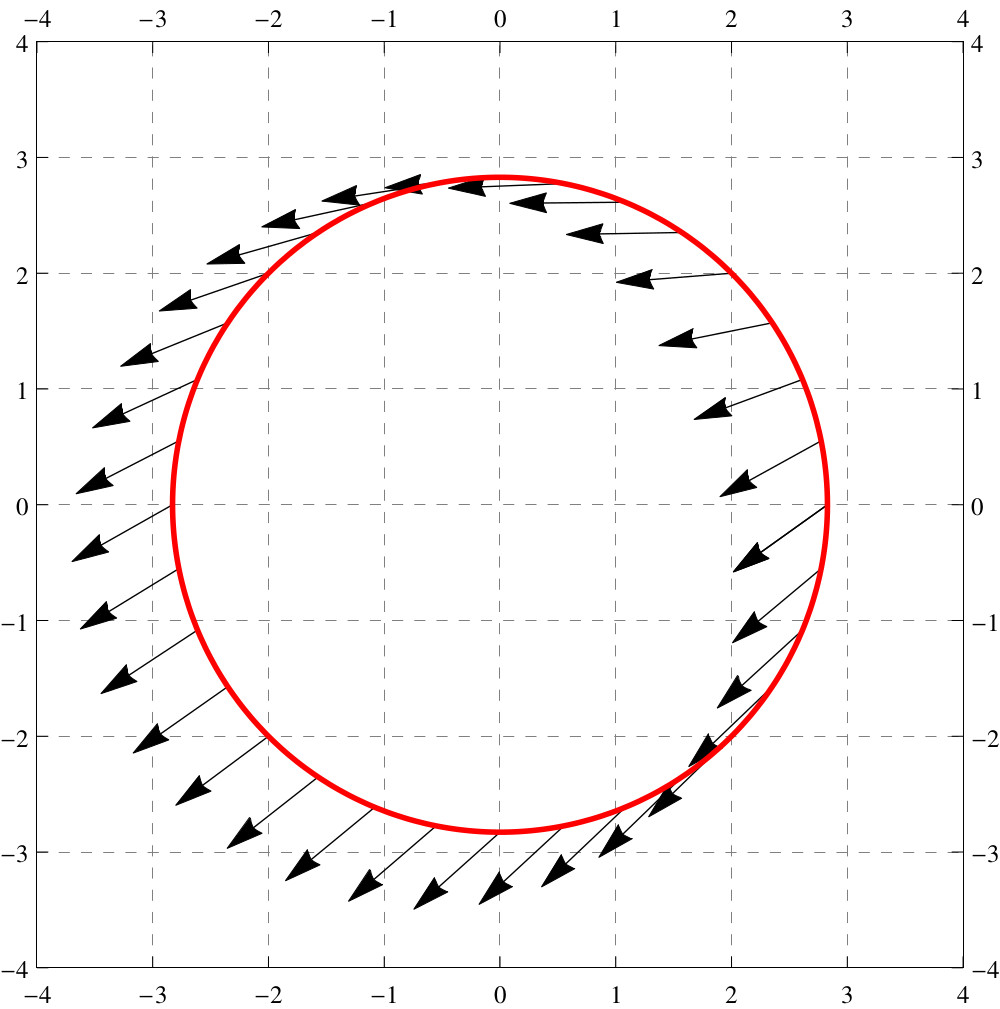
\includegraphics{curveVectors2.jpg}
  \end{image}
  Find the candidates for the maximum and minimum values for $F$ when
  restricted to $G(x,y) = c$.
  \begin{explanation}
    At the candidates for the extrema, we know that the gradient
    vector of $F$ must be
    \wordChoice{\choice{parallel}\choice[correct]{perpendicular}} to
    the curve $G(x,y) = c$. Hence we see that the points
    \[
    (x,y)\approx\left(\answer[given,tolerance=.3]{2.6},\answer[given,tolerance=.3]{1}\right)
    \]
    and
    \[
    (x,y)\approx \left(-2.3,\answer[given,tolerance=.3]{-1.6}\right)
    \]
    are our candidates for extrema.
    \begin{feedback}[correct]
      At these points,
      \begin{image}
        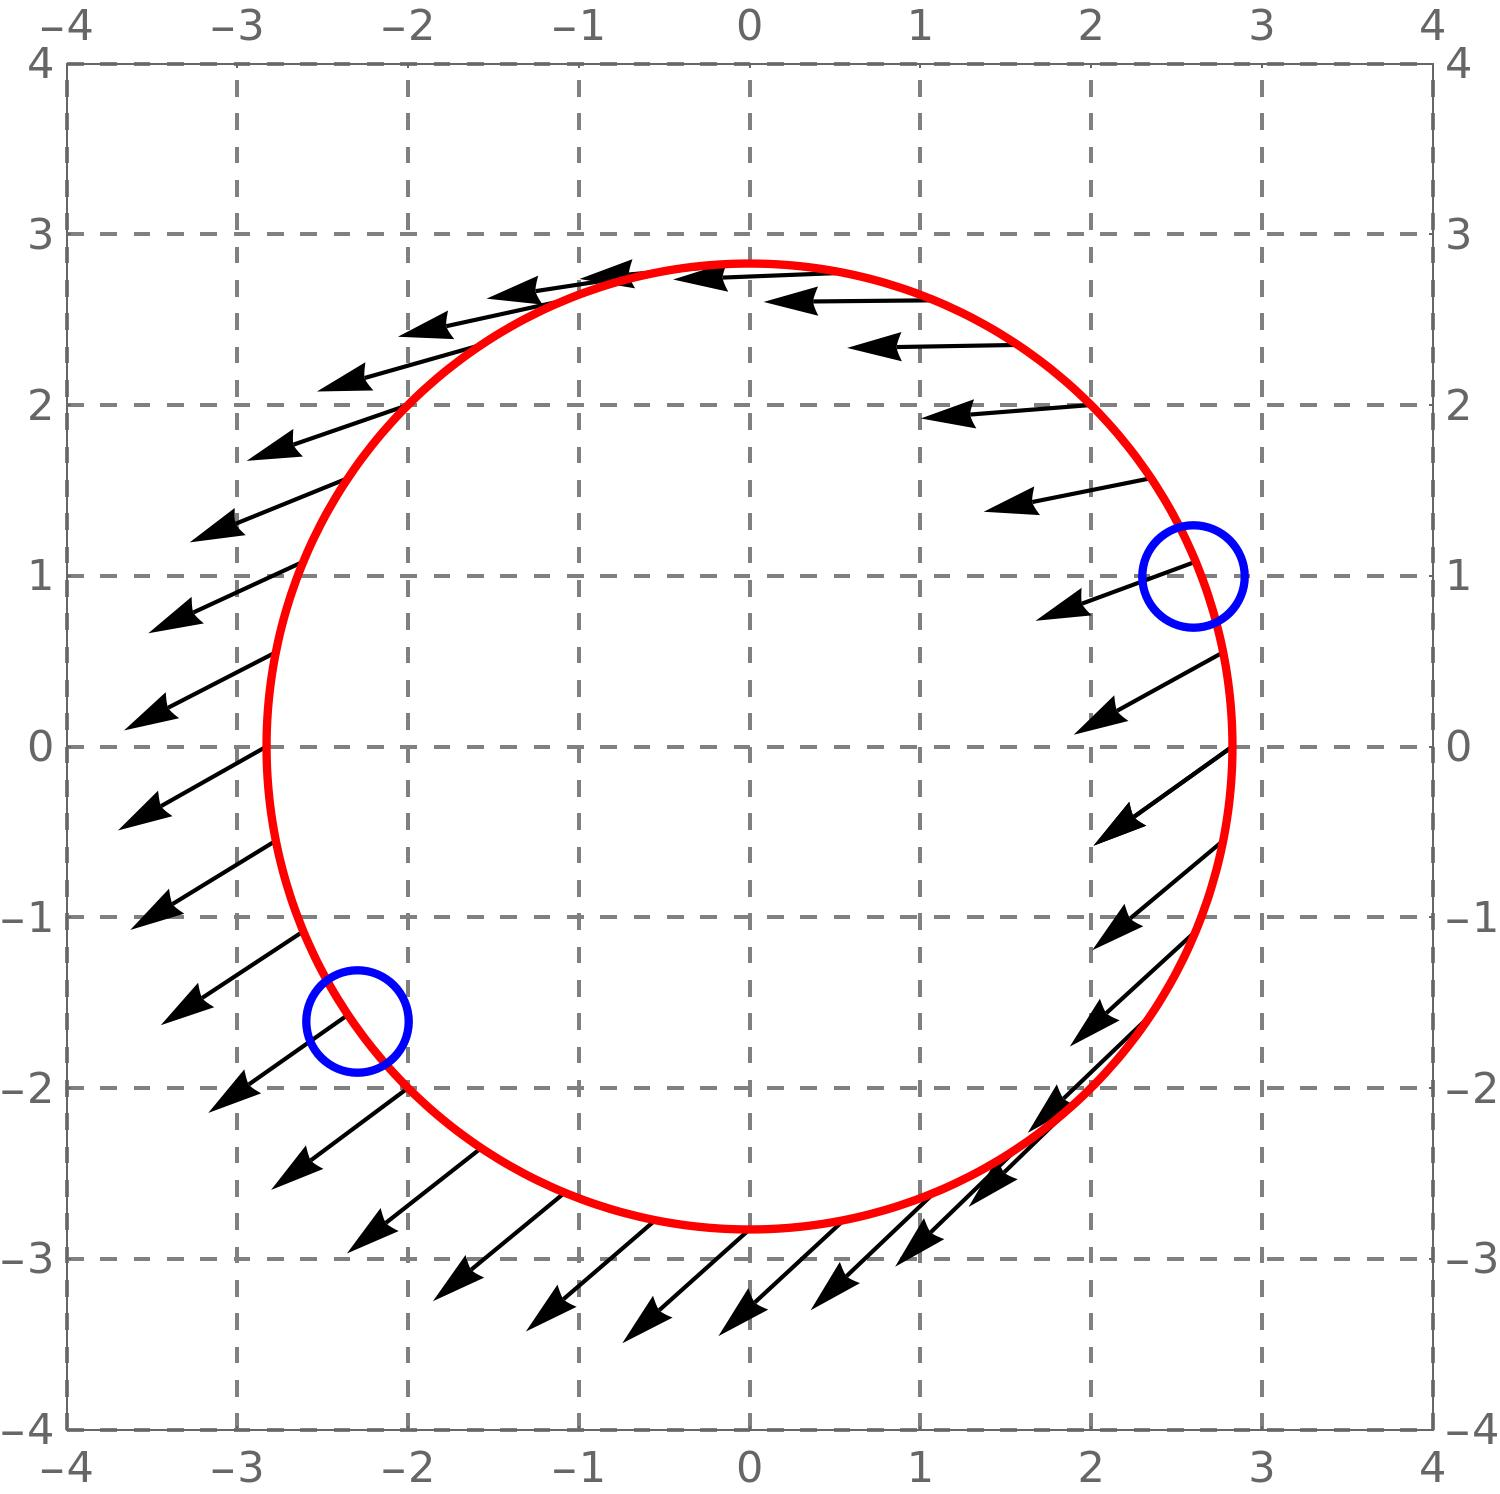
\includegraphics{curveVectors2Feedback.jpg}
      \end{image}
      the gradient vector for $G$ are parallel to the gradient vectors
      for $F$.
    \end{feedback}
  \end{explanation}
\end{example}

\begin{example}
  Below we have plotted a curve $G(x,y) = c$ along with $\grad F$.
  \begin{image}
    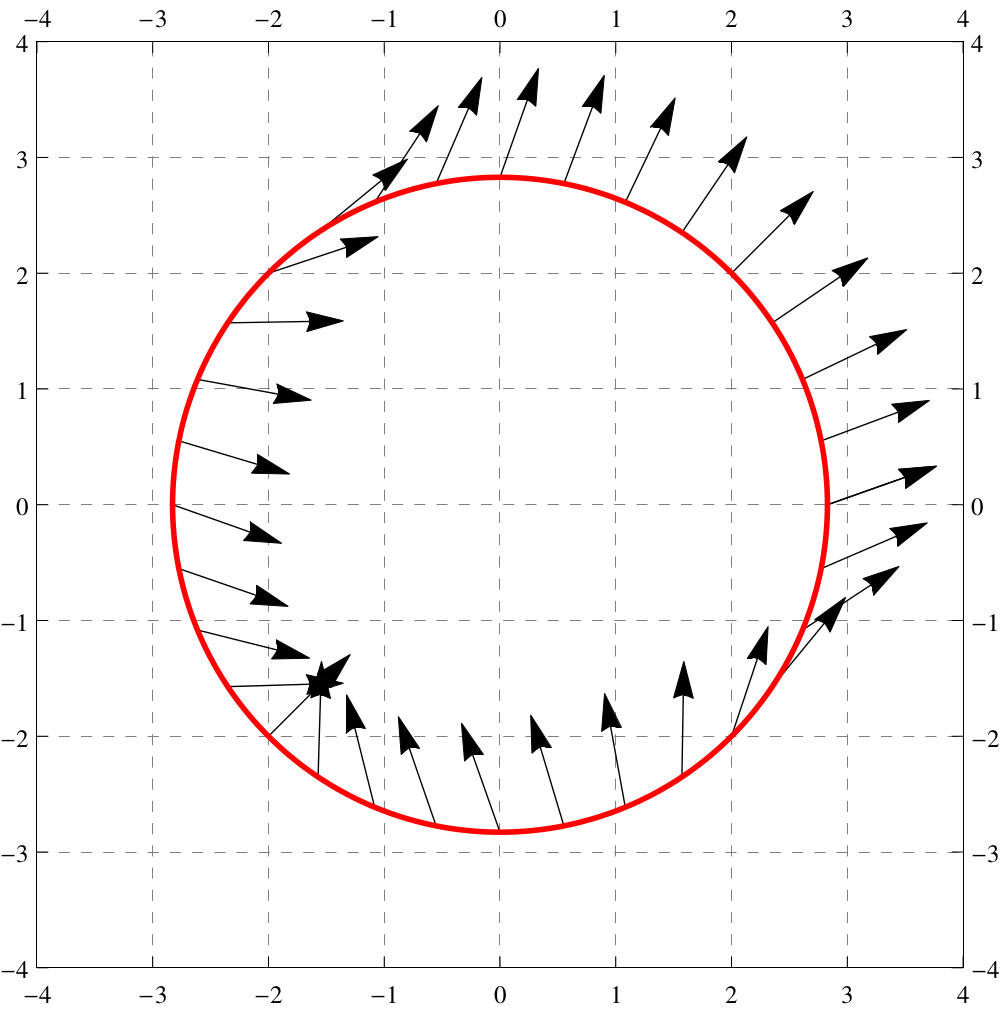
\includegraphics{curveVectors1.jpg}
  \end{image}
  Find the candidates for the maximum and minimum values for $F$ when
  restricted to $G(x,y) = c$.
  \begin{explanation}
    At the candidates for the extrema, we know that the gradient
    vector of $F$ must be
    \wordChoice{\choice{parallel}\choice[correct]{perpendicular}} to
    the curve $G(x,y) = c$. Hence we
    see that the points
    \begin{align*}
      (x,y) &= \left(\answer[given]{2},2\right)\\
      (x,y) &= \left(-2,\answer[given]{-2}\right)\\
      (x,y) &\approx \left(\answer[given,tolerance=.3]{0.7},-2.7\right)\\
      (x,y) &\approx \left(-2.7,\answer[given,tolerance=.3]{0.7}\right)
    \end{align*}
    are our candidates for extrema.
        \begin{feedback}[correct]
      At these points,
      \begin{image}
        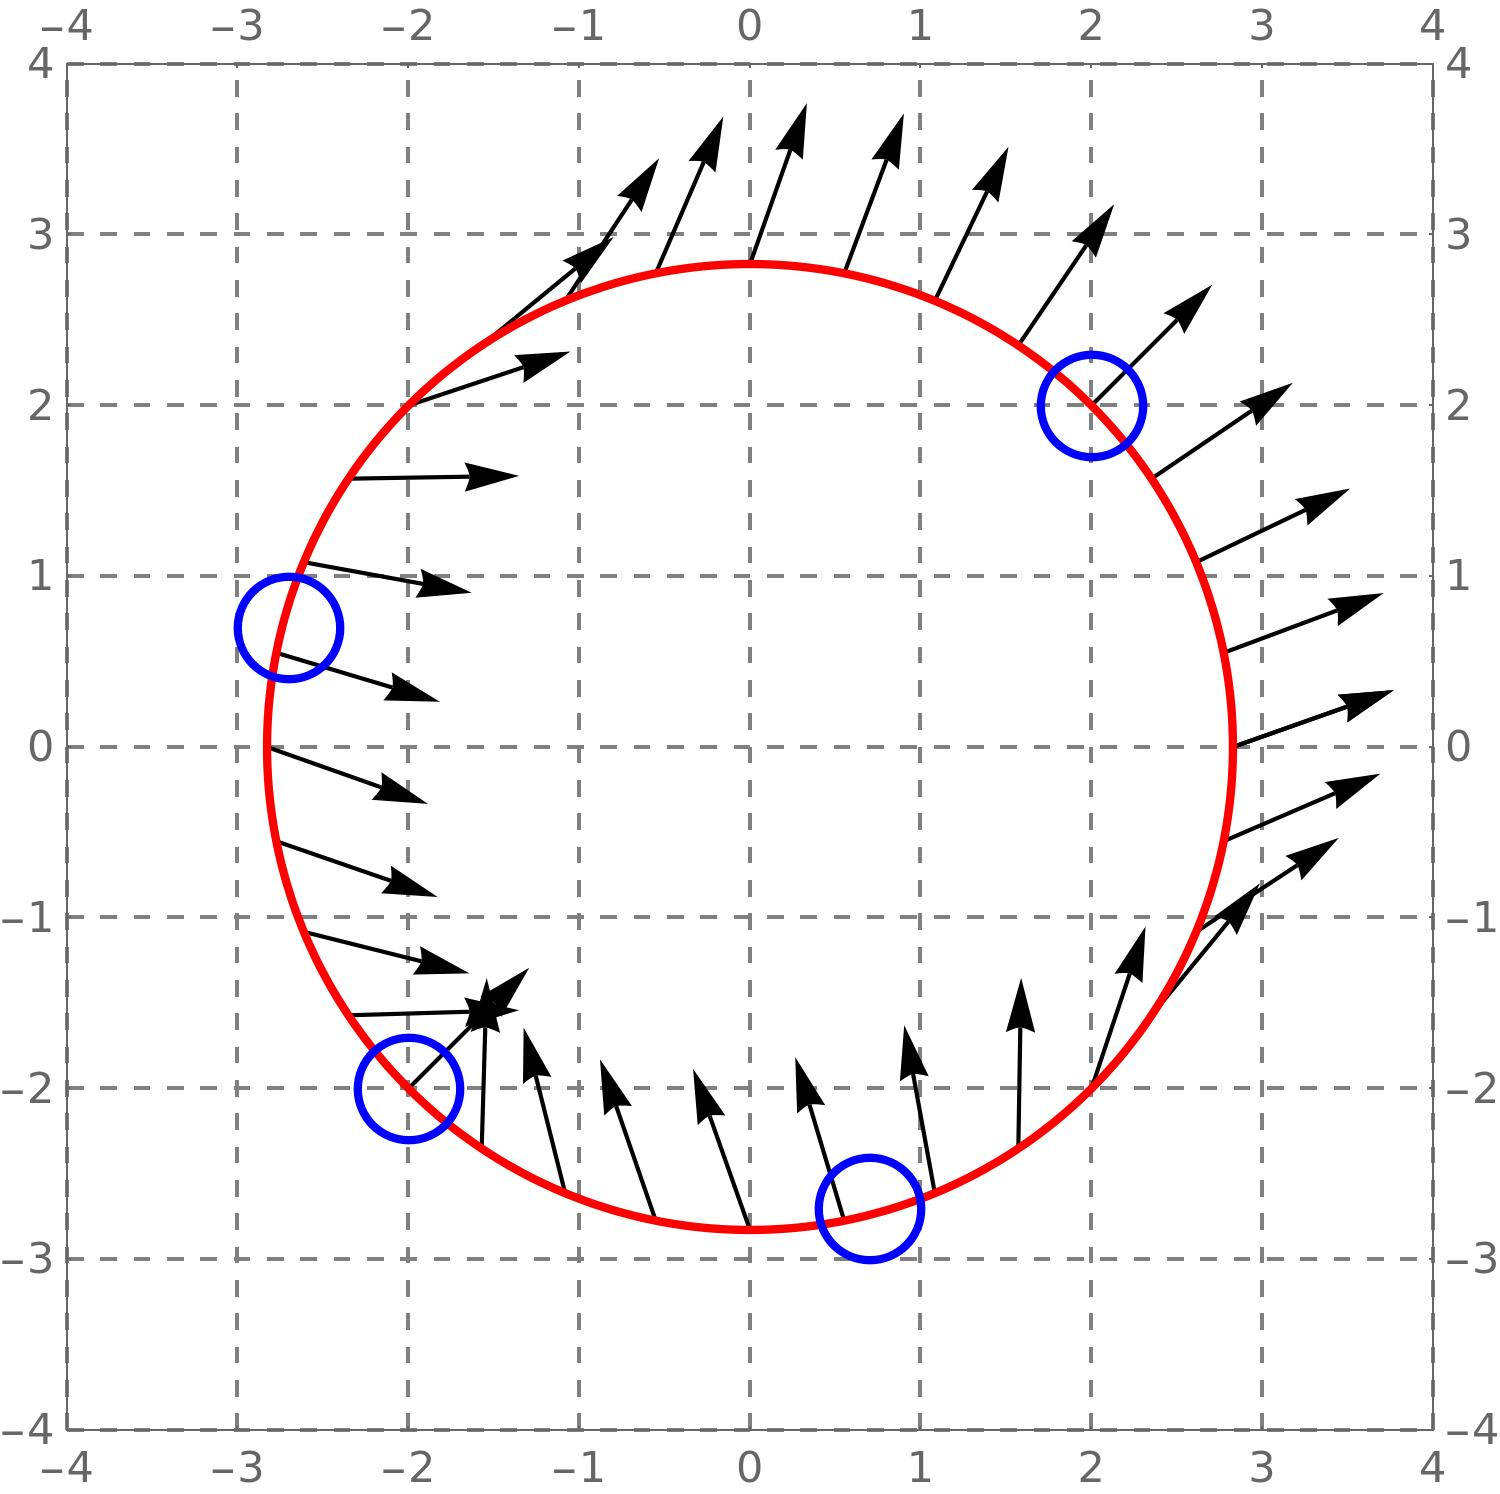
\includegraphics{curveVectors1Feedback.jpg}
      \end{image}
      the gradient vector for $G$ are parallel to the gradient vectors
      for $F$.
    \end{feedback}
  \end{explanation}
\end{example}


\section{Working with algebra}

We'll start with an example we did in our last section.

\begin{example}
Let $F(x,y) = 4x^3+4y^2-4x$ and let $C$ the set
\[
C = \{(x,y):x^2 + y^2 =1\}
\]
Find the maximum and minimum values of $F$ on $C$.
\begin{explanation}
  Start by setting $G(x,y) = x^2 + y^2$. The set $C$ is now the level
  curve $G(x,y) = \answer[given]{1}$. Now compute:
  \[
  \grad F(x,y) = \lambda \cdot \grad G(x,y)
  \]
  Write with me:
  \[
  \vector{\answer[given]{12x^2-4},\answer[given]{8y}} = \lambda \cdot \vector{\answer[given]{2x},\answer[given]{2y}}
  \]
  Breaking this vector equation into components, and adding in the constraint
  equation, the method of Lagrange multipliers gives us three
  equations and three unknowns:
  \begin{align*}
    \answer[given]{12x^2-4} &= \lambda 2x\\
    \answer[given]{8y} &= \lambda 2y\\
    \answer[given]{x^2 + y^2} &= 1
  \end{align*}
  To solve this system of equations, first note that if $y = 0$, then
  $x=\pm \answer[given]{1}$. This gives us two candidates for extrema:
  \[
  \left(1,\answer[given]{0}\right) \quad \text{and}\quad \left(-1,\answer[given]{0}\right)
  \]
  Now proceed assuming that $y\ne 0$. Looking at the second equation
  \[
  8y = \lambda 2y
  \]
  we can divide both sides by $2y$ to see that $\lambda = \answer[given]{4}$. Now we see that:
  \begin{align*}
    12x^2-4 &= \answer[given]{8x}\\
    3x^2-2x-1 &=0
  \end{align*}
  Solving this quadratic equation for $x$ we find
  \[
  x = \answer[given]{-1/3} \quad\text{and}\quad x = 1
  \]
  Now use the constraint equation $x^2 + y^2 =1$ to find $y$-values.
  From this we gain two more candidate for an extrema:
  \[
  \left(\frac{-1}{3},\answer[given]{\frac{-\sqrt{8}}{3}}\right) \quad\text{and}\quad\left(\answer[given]{\frac{-1}{3}},\frac{\sqrt{8}}{3}\right)
  \]
  Plugging these points back into $F$, we find that the minimum value of $F$ on $C$
  is $\answer[given]{0}$ and the maximum value is
  $\answer[given]{128/27}$.
\end{explanation}
\end{example}


Lagrange multipliers help out when when constraint set is given by an
implicit function. Let's see this in an example.


\begin{example}
Let $F(x,y) = x^2+2y^2-28x+51$ and let $M$ the set
\[
M = \{(x,y):y^2=x^3+1\}
\]
Find the maximum and minimum values of $F$ on $M$.
\begin{explanation}
  Start by setting $G(x,y) = x^3+1-y^2$. The set $M$ is now the level
  curve $G(x,y) = 0$. Now compute:
  \[
  \grad F(x,y) = \lambda \cdot \grad G(x,y)
  \]
  Write with me:
  \[
  \vector{\answer[given]{2x-28},\answer[given]{4y}} = \lambda \cdot \vector{\answer[given]{3x^2},\answer[given]{-2y}}
  \]
  Breaking this vector equation into components, and adding in the constraint
  equation, the method of Lagrange multipliers gives us three
  unknowns:
  \begin{align*}
    2x-28 &= \lambda 3x^2\\
    4y &= -\lambda 2y\\
    \answer[given]{x^3 + 1} &= y^2
  \end{align*}
  To solve this system of equations, first note that if $y = 0$, then
  $x=\answer[given]{-1}$. This gives us our first candidate for an extrema:
  \[
  \left(\answer[given]{-1},\answer[given]{0}\right)
  \]
  Now proceed assuming that $y\ne 0$. Looking at the second equation
  \[
  4y = -\lambda 2y
  \]
  we can divide both sides by $-2y$ to see that $\lambda = \answer[given]{-2}$. Now we see that:
  \begin{align*}
    2x-28&= -6x^2\\
    3x^2+x-14 &=0
  \end{align*}
  Solving this quadratic equation for $x$ we find
  \[
  x = \answer[given]{-7/3} \quad\text{and}\quad x = 2
  \]
  Now use the constraint equation $x^3+1=y^2$ to find $y$-values. If
  $x$ is $\answer[given]{-7/3}$, then $y$ is not a real number, so we will discard
  this solution. If $x=\answer[given]{2}$, then $y=\pm \answer[given]{3}$.  From this we gain two more
  candidate for an extrema:
  \[
  \left(\answer[given]{2},\answer[given]{-3}\right) \quad\text\quad\left(2,3\right)
  \]
  Plugging these points back into $F$, we find that the minimum value
  of $F$ on $M$ is $\answer[given]{17}$ and the maximum value is
  $\answer[given]{80}$.
\end{explanation}
\end{example}

\begin{remark}
  The constraint curve used in the example above is called a \link[Mordell curve]{https://en.wikipedia.org/wiki/Mordell_curve}. The Mordell curve is a type of \link[elliptic curve]{https://en.wikipedia.org/wiki/Elliptic_curve}, a central object of study in number theory and cryptography. For much more information on the Mordell curve, see \link[this paper by Keith Conrad]{http://www.math.uconn.edu/~kconrad/blurbs/gradnumthy/mordelleqn1.pdf}. 
\end{remark}



%% Another good example:
%% E is defined by the ellipic curve x^3-x=y^2
%% F is F(x,y) = x^2-y^2-2x

The method of Lagrange multipliers gives a unified method for solving a
large class of constrained optimization problems, and hence is used in
many areas of applied mathematics.


%% \section{The Lagrangian}

%% Finally, we should point our that there are other ways to view
%% Lagrange multipliers.

%% \begin{definition}
%%   Given functions $F:\R^n\to\R$ and $G:\R^n\to\R$ the \dfn{Lagrangian} is the function
%%   \[
%%   \mathcal{L}(\vec{x},\lambda) = F(\vec{x}) - \lambda \cdot G(\vec{x}).
%%   \]
%% \end{definition}

%% Thus to check whether
%% \[
%% \grad F(\vec{x}) = \lambda \cdot \grad G(\vec{x})
%% \]
%% is equivalent to checking where
%% \[
%% \grad \mathcal{L}(\vec{x},\lambda) = \vec{0}
%% \]
%% or has undefined components. When working with constrained
%% optimization problems by hand, the Lagrangian doesn't help much, since
%% your next step is to look at 
%% \[
%% \grad \mathcal{L}(\vec{x},\lambda) = \vec{0}.
%% \]
%% However, there are certain advantages to working with the Lagrangian:
%% \begin{itemize}
%% \item If you are working with a computer, it might be better to work
%%   in terms of the Lagrangian, as there are efficient algorithms for
%%   checking when the gradient of the function is zero.
%% \item Working with the Lagrangian gives a method for changing
%%   ``constrained'' optimization to ``unconstrained'' optimization, as
%%   we are simply finding the critical points of
%%   $\mathcal{L}(\vec{x},\lambda)$.
%% \item The Lagrangian shows us a symmetry between $F$ and $G$.
%% \end{itemize}

For some interesting extra reading check out:
\begin{itemize}
\item \link[\textit{Unifying a Family of Extrema Problems},
  W.\ Barnier and D.\ Martin, College Math Journal, November
  1997]{http://www.jstor.org/stable/2687071}.
\item \link[\textit{An ``Extremely'' Cautionary Tale}, M.\ Krusemeyer, College Math Journal, March 2000]{http://www.jstor.org/stable/2687586}.
\item \link[\textit{Lagrange Multipliers Can Fail to Determine
    Extrema}, J.\ Nunemacher, College Math Journal, January
  2003]{http://www.jstor.org/stable/3595848}.
\item \link[\textit{On the Genesis of the Lagrange Multipliers}, P.\ Bussotti, Journal of Optimization Theory and Applications, June 2003]{http://rdcu.be/HZWI}.
\end{itemize}







\end{document}





